\section{Workflow}
Figure \ref{fig:workflow} shows the general workflow of our approach towards Boolean Function Synthesis.
1. Get the continuous equivalent of boolean specification, 2. Perform Sampling over input and output variables to obtain the trainig data,
3. Train GCLN, and 4. Extract Boolean formula from the learnt Network

\begin{figure*}[t]
	\centering
    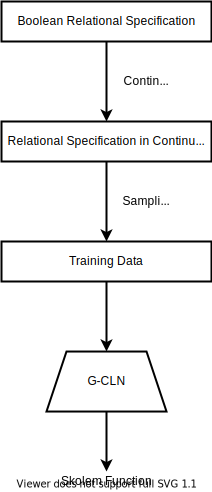
\includegraphics[scale=0.5]{workflow_bfs.png}
    \caption{Workflow}
    \label{fig:workflow}
\end{figure*}

% -------------- CODE FOR GOAL ARCHITECTURE ------------------

% \begin{figure*}
% \resizebox{!}{!}{%
% \begin{tikzpicture}[node distance=2cm]
% \node (pr) [process] {LOGICAL SPEC};
% \node (sam) [startstop, right of=pr, xshift=1.5cm] {SAMPLER};
% \node (nn) [startstop, right of=sam, xshift=2cm] {PRE-TRAINED NN FOR SKETCHES FOR A GIVEN GRAMMAR};
% \node (sol) [startstop, right of=nn, xshift=2.5cm] {SOLVER};
% \node (bs) [process, below of=nn, yshift=-0.5cm] {BAD SKETCH};
% \node (gr) [process, above of=sol, yshift=0.5cm] {GRAMMAR};
% \node (dec1) [decision, below of=sol, yshift=-0.5cm] {SOLVED?};
% \node (sn) [solution, below of=dec1, yshift=-0.5cm] {PROGRAM};
% \draw [arrow] (pr) -- node[anchor=south] {} (sam);
% \draw[-latex,bend right=45]  (pr) edge (nn);
% \draw [arrow] (sam) -- node[anchor=south] {I/O} (nn);
% \draw [arrow] (sam) -- node[anchor=north] {Examples} (nn);
% \draw [arrow] (nn) -- node[anchor=south] {SKETCHES} (sol);
% \draw [arrow] (sol) -- node[anchor=south] {} (dec1);
% \draw [arrow] (gr) -- node[anchor=south] {} (sol);
% \draw [arrow] (dec1) -- node[anchor=south] {NO} (bs);
% \draw [arrow] (bs) -- node[anchor=south] {} (nn);
% \draw [arrow] (dec1) -- node[anchor=west] {YES} (sn);
% \end{tikzpicture}
% }
% \caption{Synthesizing Sketches from Logical Embeddings}
% \label{fig:goal}
% \end{figure*}



%\Stanly{See where this fits in........We propose how to synthesize the dataset from existing SyGuS benchmarks.
%We propose an architecture for an NN that takes an embedding of I/O + Logical Formula and synthesizes a sketch which is expected to work better than previous approaches. The reason is because we encode the semantics of the logical spec using GNN.
%As a consequence of the above two points, we will also have a baseline approach that synthesizes complete programs from logical spec embeddings.
%Lastly, we wish to think about teaching the NN to recognise "bad sketches" which is now feasible due to this architecture.}

\subsection{Sampling Strategy}
Figure \ref{fig:sampling} describes the sampling pipeline that we have implemented to generate the training data.
Currently we are using Random Sampling Strategy in which, 
we sample uniformly at random for input and output variables in the range $[0, 1]$. 
These random samples are then applied with the continous mapping of relational specification (F). 
Output of F is then thresholded to get the positive samples. 

\begin{figure*}
	\centering
    \includegraphics[scale=0.5]{sampling_bfs.png}
    \caption{Sampling Pipeline}
    \label{fig:sampling}
\end{figure*}

Apart from Random Sampling, we also use Correlated Sampling Strategy for one of the problem formulation. 
In this strategy, we first sample the input variables and the output variables are conditioned on input variables. 
This may help to capture the correlation betweenn input and output variables.

\begin{table}[t]
\begin{center}
\begin{tabular}{cccc}
	x: & y: & XOR(x, y)\\ 
	0.9 & 0.2 & 0.72 \\  
	0.85 & 0.01 & 0.84
\end{tabular}
\caption{Example Samples for XOR(x, y) with threshold = 0.7 and Product t-norm}
\label{tab:tnorms}
\end{center}
\end{table}


\subsection{GCLN Architecture}

% Figure \ref{fig:goal} describes the high level idea for synthesizing sketches from logical embeddings. We first sample a finite set of I/O examples from the logical specification. We wish to have a pre trained neural network for a given DSL that is trained to generate the required sketches when a logical specification and I/O specification are given as input. As a novel extension, it may also be possible for the NN to take as input a bad sketch and make decisions accordingly. This would be something similar to CEGIS(T) but using an NN. We then feed it to a traditional solver that solves the sketch using enumerative techniques if the sketch has non constant holes and constraint based techniques, if the sketch has constant holes. If the sketch is infeasible, then we use this to direct our NN to synthesize a better sketch. The meaning of an infeasible sketch is that there does not exist a valid (w.r.t. the DSL) completion of the sketch for the given specification.

% The major research question here is how to make the NN understand whether a given sketch is an infeasible sketch or not.